\documentclass[11pt]{beamer}
\usetheme{Madrid}

\usepackage[T1]{fontenc}
\usepackage{lmodern}
\usepackage[sanserif]{complexity}
\usepackage{twemojis}


\usepackage{algpseudocode}

\usepackage{tikz}
\usetikzlibrary{arrows.meta, positioning, shapes.geometric,
                fit, backgrounds, calc}
 
\tikzset{
  stepbox/.style={
    rectangle, rounded corners=5pt,
    minimum width=3.8cm, minimum height=1.0cm,
    align=center, font=\small\bfseries,
    inner sep=6pt, draw, very thick,
  },
  refbox/.style={stepbox, draw=black, fill=white, text=black},
  selbox/.style={stepbox, draw=black, fill=white, text=black},
  invbox/.style={stepbox, draw=black, fill=white, text=black},
  mainarrow/.style={-{Stealth[length=7pt]}, line width=1.4pt},
  looparrow/.style={-{Stealth[length=6pt]}, line width=1.1pt, dashed, color=black},
  every picture/.append style={node distance=1.2cm and 1.6cm},
}

\usepackage{svg}
\usepackage{amsmath}
\usepackage{amsfonts}
\usepackage{amssymb}
\usepackage{graphicx}
\usepackage{adjustbox}
\usepackage{tikz}
\usetikzlibrary{positioning}
\usetikzlibrary{calc}

\usepackage{xcolor}

\definecolor{cTriangle}{HTML}{D62728}   % tab:red
\definecolor{cPaths}{HTML}{2CA02C}      % tab:green
\definecolor{cTriple}{HTML}{1F77B4}     % tab:blue
\definecolor{cNauty}{HTML}{BDB76B}      % darkkhaki

% Un item de légende générique : couleur, symbole, étiquette
\newcommand{\legenditem}[3]{{\color{#1}#2}~#3}

\newcommand{\legendeInvariants}{%
  \begin{center}
  \Large
  \legenditem{cTriangle}{$\blacktriangle$}{triangle}\quad
  \legenditem{cPaths}{$\blacklozenge$}{paths}\quad
  \legenditem{cTriple}{$\bullet$}{triple}\quad
  \legenditem{cNauty}{$\boldsymbol{\times}$}{\textit{Nauty}}
  \end{center}
}

\definecolor{mydarkgray}{gray}{0.25} % 0=noir, 1=blanc



\definecolor{leafA}{HTML}{E63946} % feuille 1
\definecolor{leafB}{HTML}{2A9D8F} % feuille 2
\definecolor{leafC}{HTML}{264653} % feuille 3


\newcommand{\Kautoexample}[4]{%
  \begin{tikzpicture}[baseline=(current bounding box.center),
      vtx/.style={circle,draw,minimum size=5mm,inner sep=0pt}]
    \node[vtx,fill=black!70]  (c) at (0,0)          {};
    \node[vtx,fill=#1]        (t) at (0,0.9)         {};
    \node[vtx,fill=#2]        (l) at (-0.78,-0.45)   {};
    \node[vtx,fill=#3]        (r) at (0.78,-0.45)    {};
    \draw[thick] (c) -- (t);
    \draw[thick] (c) -- (l);
    \draw[thick] (c) -- (r);
    \node at (0,-1.15) {\footnotesize $#4$};
  \end{tikzpicture}%
}
  
\DeclareMathOperator{\sen}{sen}
\DeclareMathOperator{\tg}{tg}

\setbeamertemplate{caption}[numbered]

\author[Rodolphe Prévot]{
        Auteur: Rodolphe Prévot\\
        Promoteur: Robin Petit\\
        Directeur: Gwenaël Joret
}

\title[Défense Mémoire]{Canonical Labelling and Graph
Isomorphism: A C++ Reimplementation
of Nauty}

\newcommand{\email}{rodolphe.prevot@ulb.be}

\setbeamertemplate{navigation symbols}{} 
\logo{
\includegraphics[scale=0.03]{imgs/titlepage/sceau-a-quadri.jpg}} 
\institute[]{Université libre de Bruxelles \par Département d’Informatique} 
\date{Septembre 2026} 

\bibliographystyle{apalike}

\begin{document}


\AtBeginSection[]{
\begin{frame}[plain]

\begin{tikzpicture}[remember picture,overlay]

    % Bande bleue
    \fill[blue!70!black]
        ([yshift=-3.2cm]current page.north west)
        rectangle
        ([yshift=-5.4cm]current page.north east);

    % Titre centré dans la bande
    \node[
        text=white,
        align=center
    ] at ([yshift=-4.3cm]current page.north)
    {
        \adjustbox{max width=0.9\paperwidth}{
            \bfseries\fontsize{26}{30}\selectfont
            \insertsection
        }
    };

    % Logo ULB
    % Logo ULB sous la bande
\node at ([yshift=-2.2cm]current page.center)
{
    
\includegraphics[height=1.6cm]{imgs/titlepage/sceau-a-quadri.jpg}
};

\end{tikzpicture}

\end{frame}
}

\begin{frame}
\titlepage\end{frame}


\setbeamertemplate{logo}{}

\begin{frame}{Sommaire}
\tableofcontents 
\end{frame}

\section{Contexte}

\begin{frame}{Isomorphisme}
    \begin{columns}[c] % [c] = alignement vertical centré des colonnes
        % --- Image de gauche ---
        \begin{column}{0.42\textwidth}
            \centering
            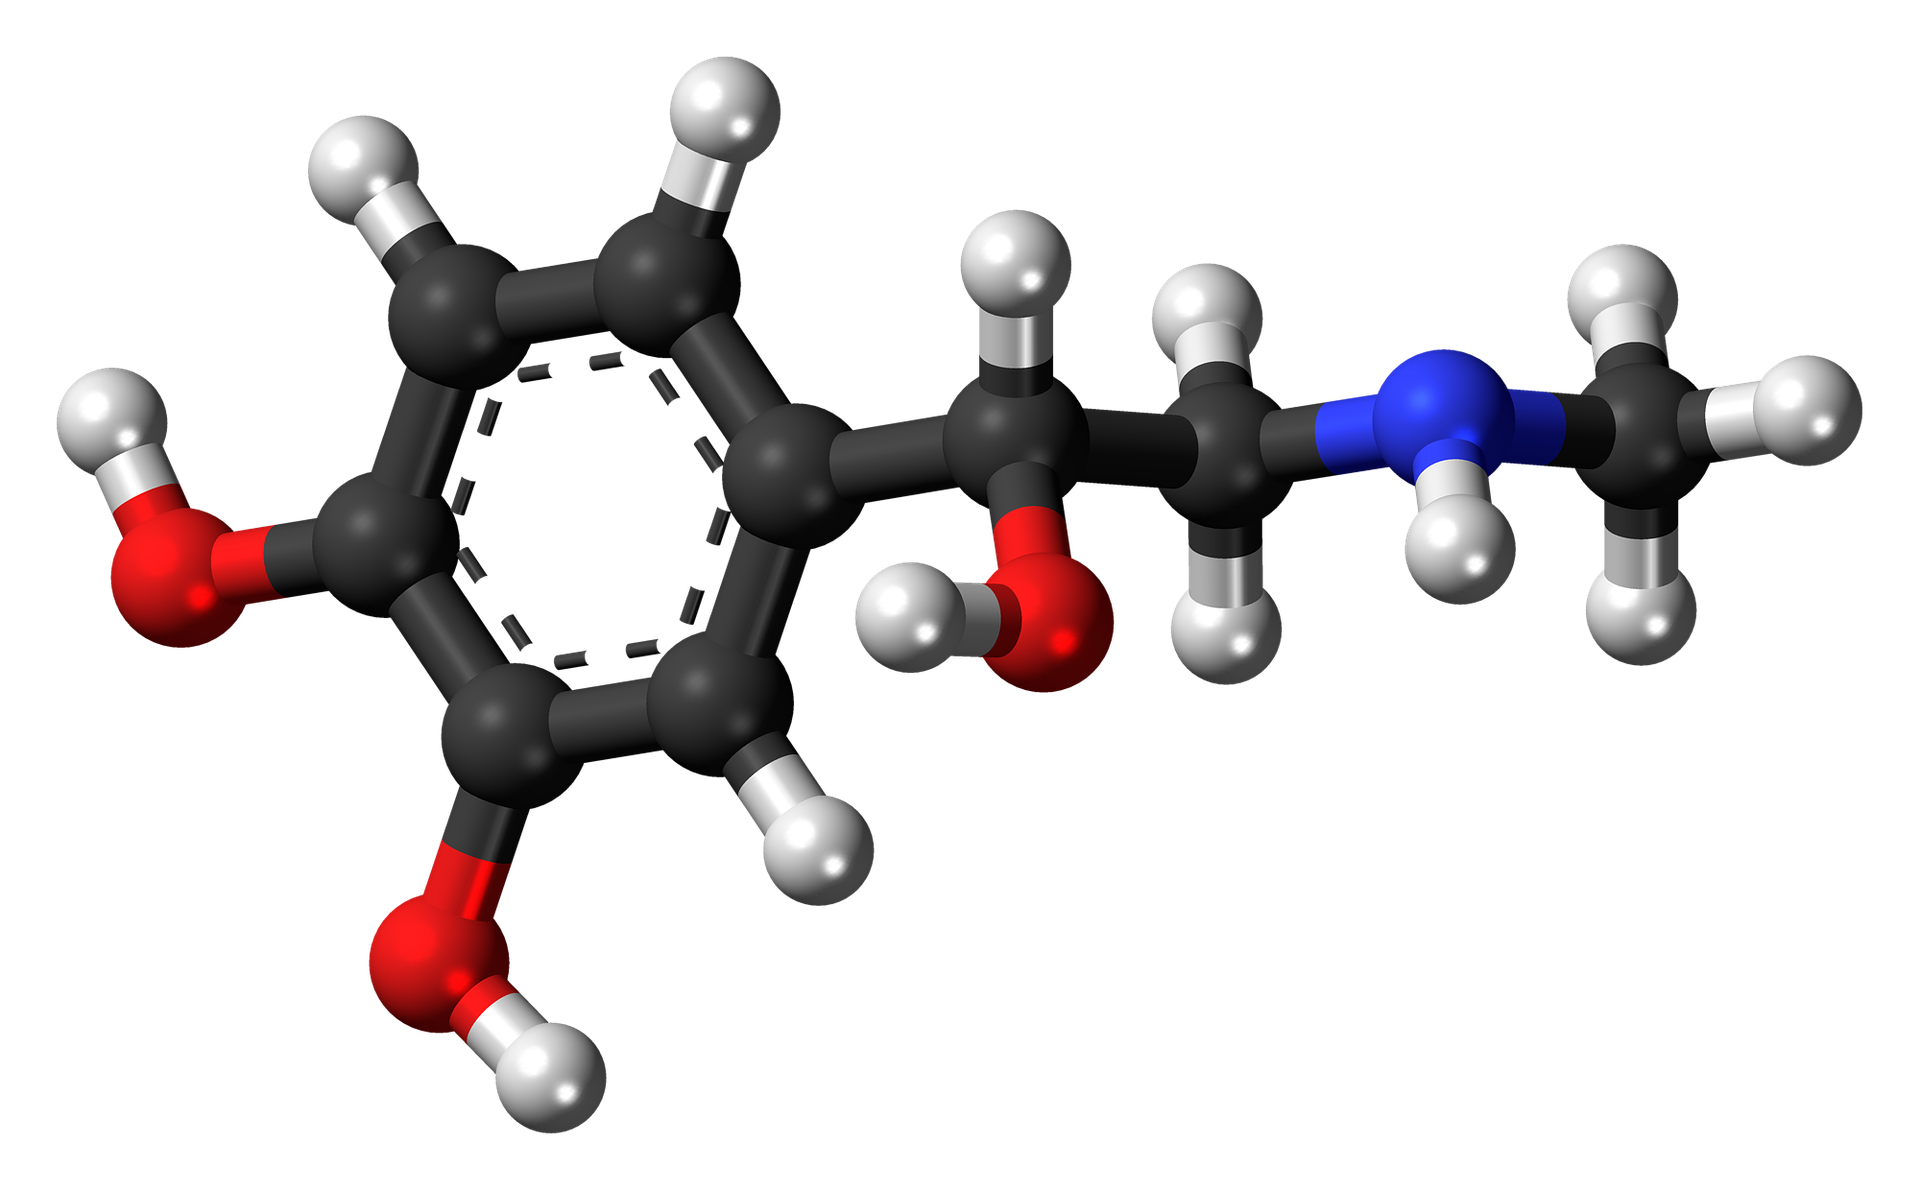
\includegraphics[width=\linewidth]{imgs/slide/wikimediaimages-adrenaline-872345_1920 (1).png}
        \end{column}
 
        % --- Symbole central ---
        \begin{column}{0.16\textwidth}
            \centering
            \Huge $\overset{?}{\cong}$
        \end{column}
        % --- Image de droite ---
        \begin{column}{0.42\textwidth}
            \centering
            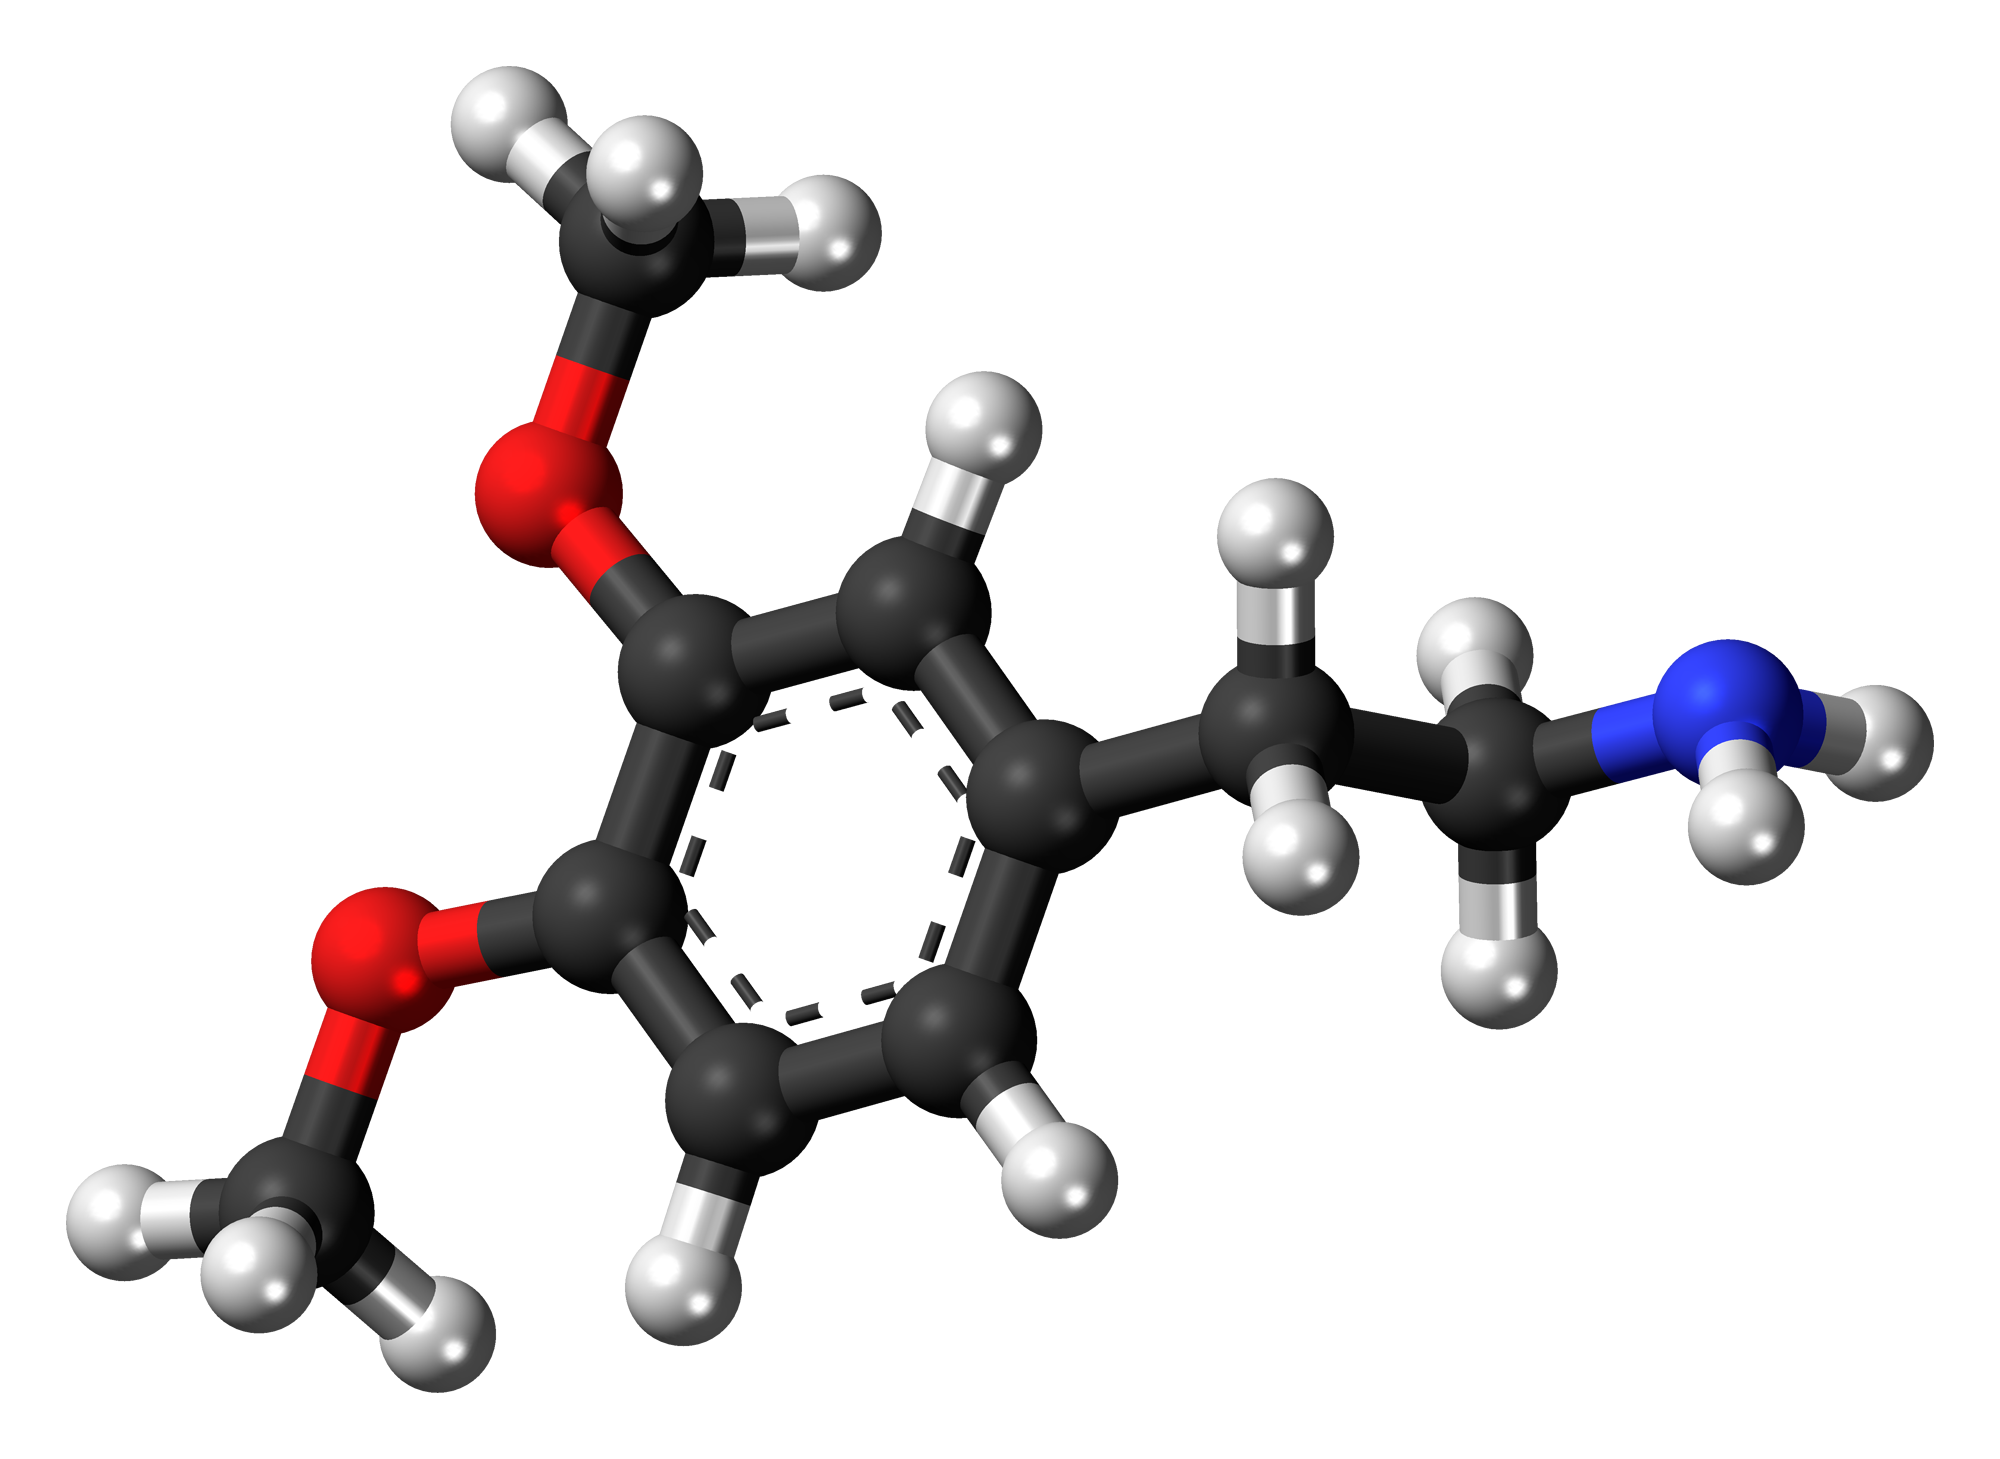
\includegraphics[width=\linewidth]{imgs/slide/wikimediaimages-dimethoxyphenethylamine-867172.png}
        \end{column}
    \end{columns}
 
    \vspace{1em}
    \centering
    \small Structurellement les mêmes?
\end{frame}

\begin{frame}{Exemple (1/2)}

\begin{figure}[h!]
    \centering
    \resizebox{0.9\textwidth}{!}{%
    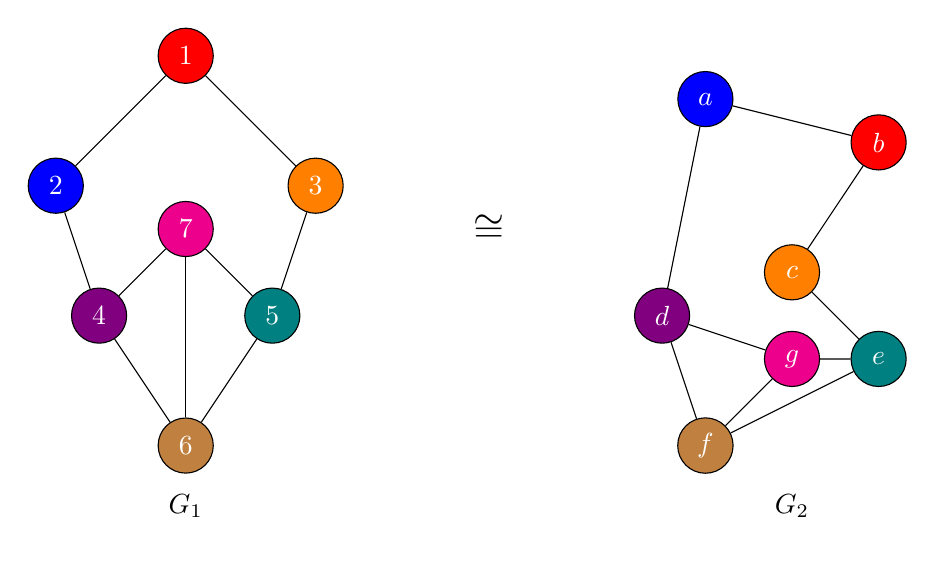
\begin{tikzpicture}[
    scale=1.1,
    every node/.style={circle, draw, minimum size=7mm}
]

\tikzset{iso/.style={fill=#1, draw=black, text=white}}

% ================= G1 =================

\node[iso=red]     (v1) at (0,2.5)   {$1$};
\node[iso=blue]    (v2) at (-1.5,1)  {$2$};
\node[iso=orange]  (v3) at (1.5,1)   {$3$};
\node[iso=violet]  (v4) at (-1,-0.5) {$4$};
\node[iso=teal]    (v5) at (1,-0.5)  {$5$};
\node[iso=brown]   (v6) at (0,-2)    {$6$};
\node[iso=magenta] (v7) at (0,0.5)   {$7$};

\draw (v1)--(v2);
\draw (v1)--(v3);
\draw (v2)--(v4);
\draw (v3)--(v5);
\draw (v4)--(v6);
\draw (v5)--(v6);
\draw (v4)--(v7);
\draw (v5)--(v7);
\draw (v6)--(v7);

\node[draw=none, rectangle] at (0,-2.7) {$G_1$};


% ================= G2 =================
% même couleur = même sommet sous f

\node[iso=blue]    (u1) at (6,2)      {$a$};
\node[iso=red]     (u2) at (8,1.5)    {$b$};
\node[iso=orange]  (u3) at (7,0)      {$c$};
\node[iso=violet]  (u4) at (5.5,-0.5) {$d$};
\node[iso=teal]    (u5) at (8,-1)     {$e$};
\node[iso=brown]   (u6) at (6,-2)     {$f$};
\node[iso=magenta] (u7) at (7,-1)     {$g$};

\draw (u1)--(u2);
\draw (u1)--(u4);
\draw (u2)--(u3);
\draw (u3)--(u5);
\draw (u4)--(u6);
\draw (u5)--(u6);
\draw (u4)--(u7);
\draw (u5)--(u7);
\draw (u6)--(u7);

\node[draw=none, rectangle] at (7,-2.7) {$G_2$};


% ================= Symbole d'isomorphisme =================

\node[draw=none, rectangle] at (3.5,0.5) {\Large $\cong$};

\end{tikzpicture}%
    }
    \caption{Isomorphisme}
    \end{figure}

\end{frame}


\begin{frame}{Exemple (2/2)}

    \begin{figure}[h!]
        \centering
        \resizebox{0.9\textwidth}{!}{%
        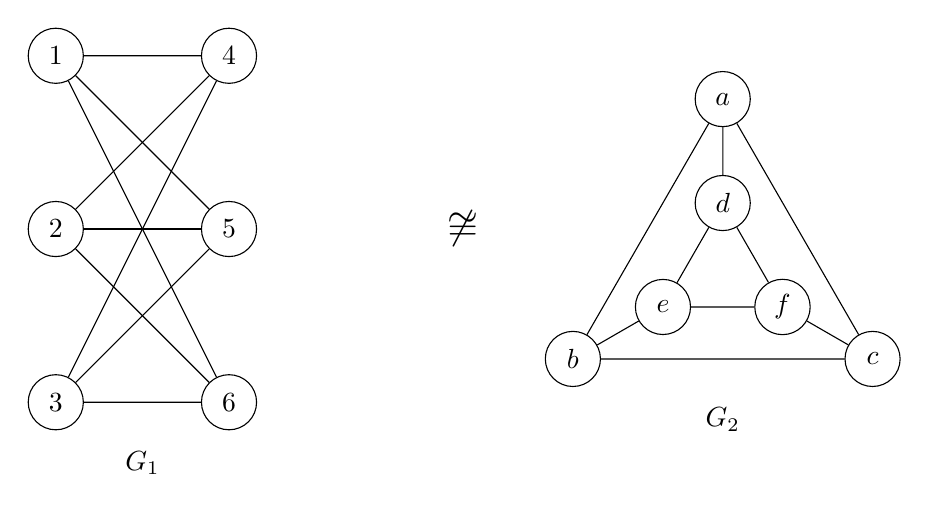
\begin{tikzpicture}[
    scale=1.1,
    every node/.style={circle, draw, minimum size=7mm}
]


% ================= G1 : K_{3,3} =================

\node (v1) at (-0.7,2)  {$1$};
\node (v2) at (-0.7,0)  {$2$};
\node (v3) at (-0.7,-2) {$3$};

\node (v4) at (1.3,2)   {$4$};
\node (v5) at (1.3,0)   {$5$};
\node (v6) at (1.3,-2)  {$6$};

\draw (v1)--(v4);
\draw (v1)--(v5);
\draw (v1)--(v6);

\draw (v2)--(v4);
\draw (v2)--(v5);
\draw (v2)--(v6);

\draw (v3)--(v4);
\draw (v3)--(v5);
\draw (v3)--(v6);

\node[draw=none, rectangle] at (0.3,-2.7) {$G_1$};

% ================= G2 : prisme triangulaire (recentré sur y=0) =================

\node (ua) at (7,1.5)     {$a$};
\node (ub) at (5.27,-1.5) {$b$};
\node (uc) at (8.73,-1.5) {$c$};
\node (ud) at (7,0.3)     {$d$};
\node (ue) at (6.31,-0.9) {$e$};
\node (uf) at (7.69,-0.9) {$f$};

\draw (ua)--(ub);
\draw (ub)--(uc);
\draw (uc)--(ua);
\draw (ud)--(ue);
\draw (ue)--(uf);
\draw (uf)--(ud);
\draw (ua)--(ud);
\draw (ub)--(ue);
\draw (uc)--(uf);

\node[draw=none, rectangle] at (7,-2.2) {$G_2$};

% ================= Symbole de non-isomorphisme =================

\node[draw=none, rectangle] at (4,0) {\Large $\not\cong$};

\end{tikzpicture}%
        }
        \caption{Pas d'isomorphisme}
        \end{figure}
\end{frame}

\begin{frame}{Problème général}

\begin{itemize}
    \item Problème d'isomorphisme de graphe ($\mathrm{IG}$)
    \item Complexité: \(\mathrm{IG} \in \NP,\quad \mathrm{IG} \stackrel{?}{\in} \P{},\quad \mathrm{IG} \stackrel{?}{\in} \NPC{}\)
    \item Considéré \NPI{}
    \item Meilleur algorithme quasi-polynomial: László Babai (2016)
    \item Forme canonique plus efficace en pratique (\textit{Nauty})
\end{itemize}
\end{frame}

\begin{frame}{Forme canonique}

Principe: Problème d'équivalence en problème d'égalité


\begin{figure}[H]
    \centering
    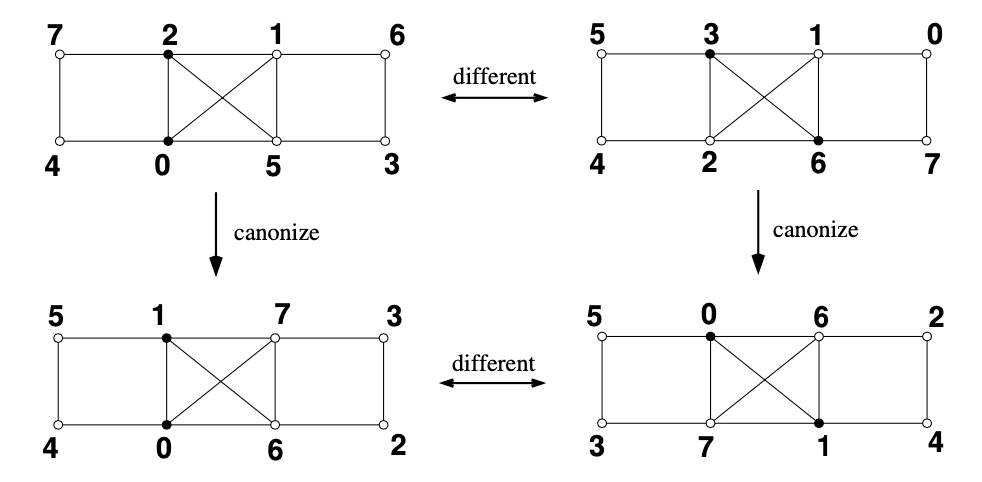
\includegraphics[width=0.8\linewidth]{imgs/pré-mémoire.png}
\end{figure}
    
\end{frame}

\section{Nauty}

\begin{frame}{Arbre de recherche}

    \begin{figure}[h!]
        \centering
        \resizebox{0.9\textwidth}{!}{%
        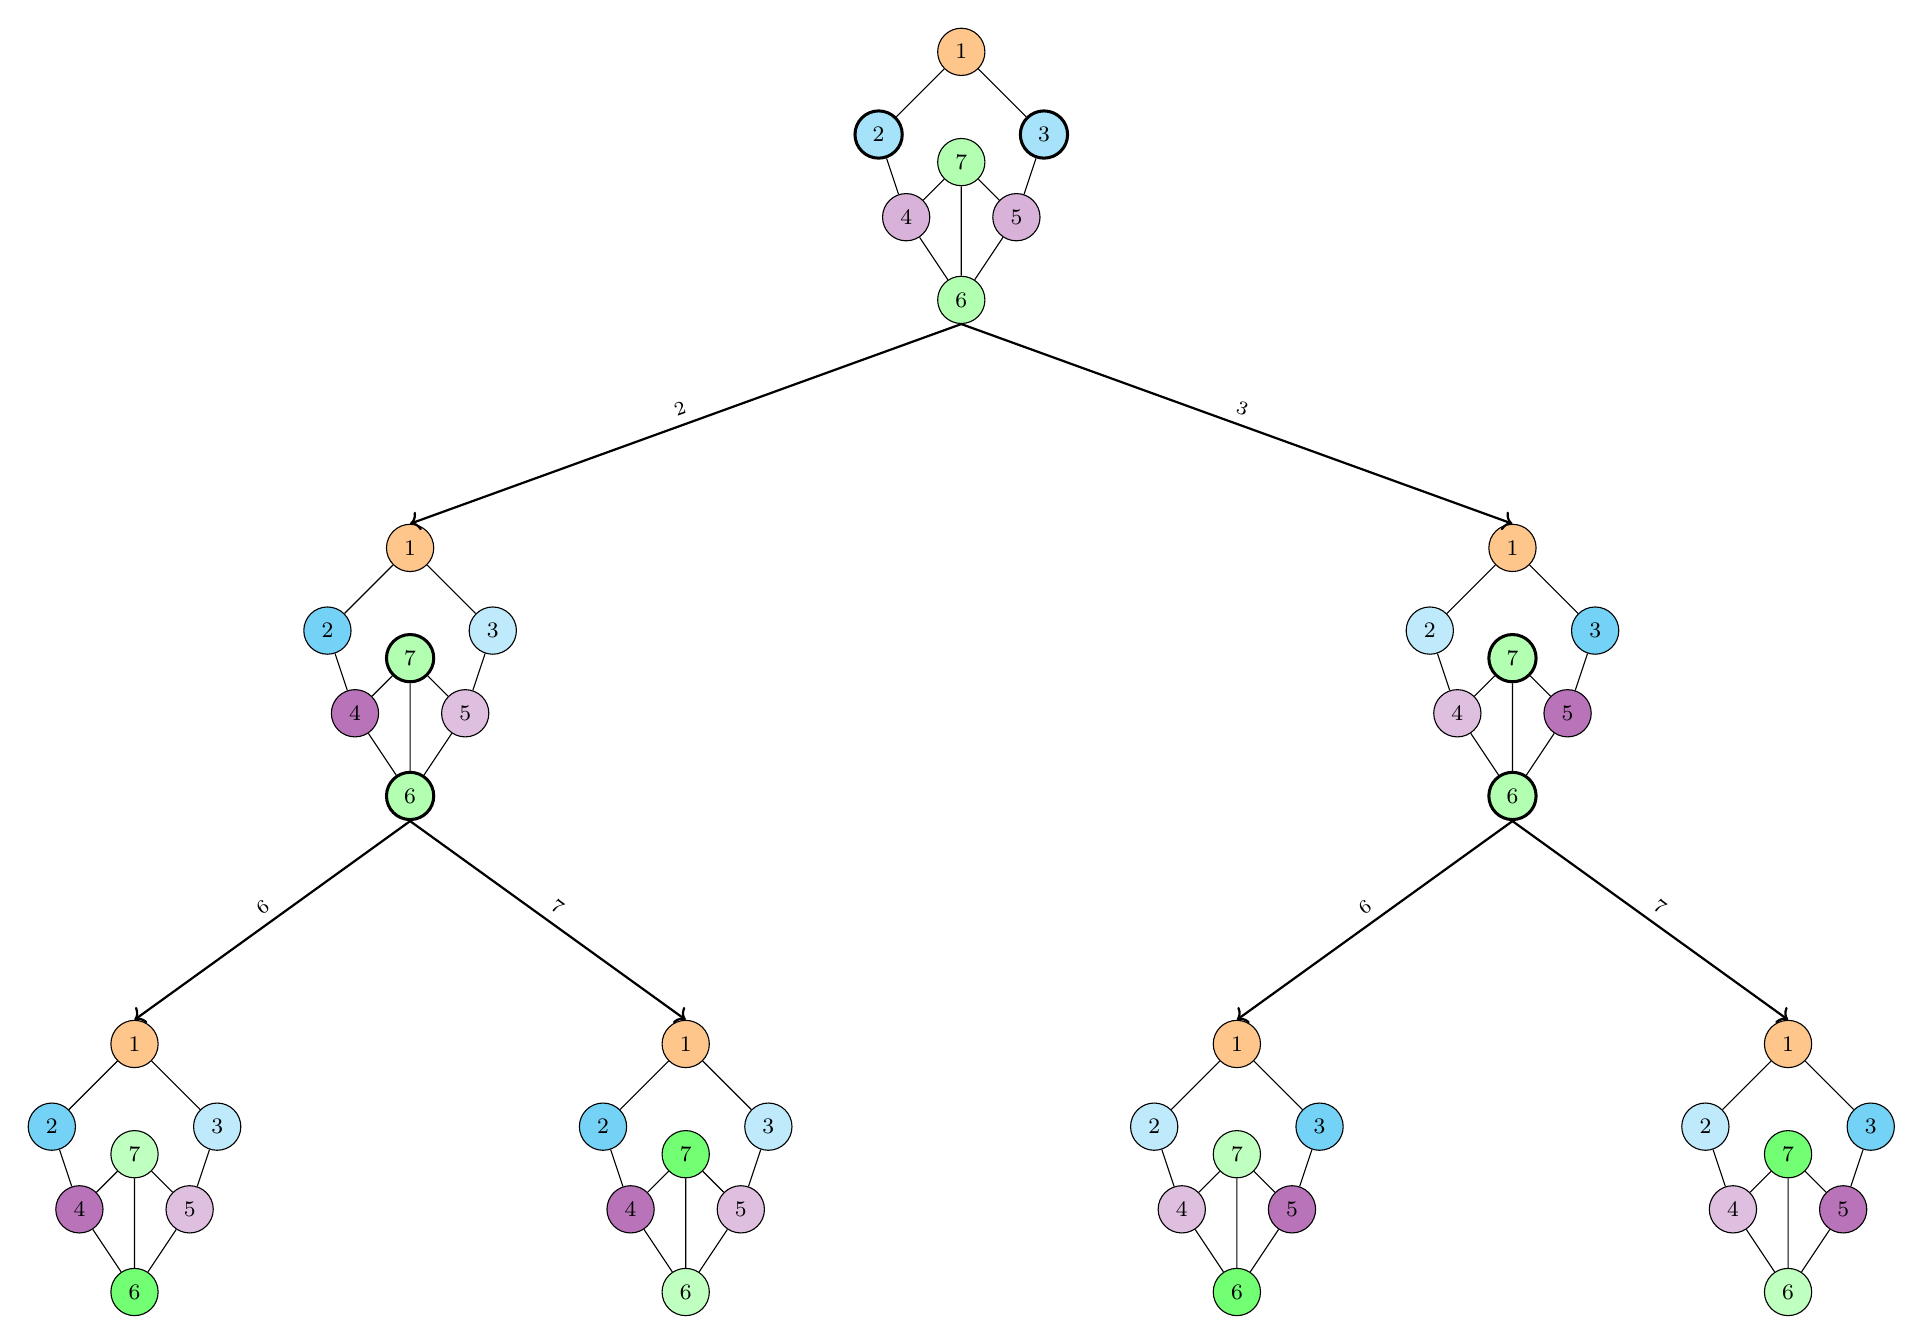
\begin{tikzpicture}[scale=0.7]

    \tikzset{
        v/.style={
            circle,
            draw,
            minimum size=6mm,
            inner sep=0pt,
            font=\footnotesize
        },
        vt/.style={
            v,
            line width=1.1pt
        }
    }

    % ============================================================
    % Niveau 0 : racine
    % ============================================================
    \begin{scope}[xshift=0cm, yshift=0cm]

        \node[v, fill=orange!45] (r1) at (0,2.5) {1};
        \node[vt, fill=cyan!35] (r2) at (-1.5,1) {2};
        \node[vt, fill=cyan!35] (r3) at (1.5,1) {3};
        \node[v, fill=violet!30] (r4) at (-1,-0.5) {4};
        \node[v, fill=violet!30] (r5) at (1,-0.5) {5};
        \node[v, fill=green!30] (r6) at (0,-2) {6};
        \node[v, fill=green!30] (r7) at (0,0.5) {7};

        \draw
            (r1)--(r2)
            (r1)--(r3)
            (r2)--(r4)
            (r3)--(r5)
            (r4)--(r6)
            (r5)--(r6)
            (r4)--(r7)
            (r5)--(r7)
            (r6)--(r7);

    \end{scope}


    % ============================================================
    % Niveau 1 gauche : individualisation de 2
    % ============================================================
    \begin{scope}[xshift=-10cm, yshift=-9cm]

        \node[v, fill=orange!45] (l1) at (0,2.5) {1};
        \node[v, fill=cyan!55] (l2) at (-1.5,1) {2};
        \node[v, fill=cyan!25] (l3) at (1.5,1) {3};
        \node[v, fill=violet!55] (l4) at (-1,-0.5) {4};
        \node[v, fill=violet!25] (l5) at (1,-0.5) {5};
        \node[vt, fill=green!30] (l6) at (0,-2) {6};
        \node[vt, fill=green!30] (l7) at (0,0.5) {7};

        \draw
            (l1)--(l2)
            (l1)--(l3)
            (l2)--(l4)
            (l3)--(l5)
            (l4)--(l6)
            (l5)--(l6)
            (l4)--(l7)
            (l5)--(l7)
            (l6)--(l7);

    \end{scope}


    % ============================================================
    % Niveau 1 droite : individualisation de 3
    % ============================================================
    \begin{scope}[xshift=10cm, yshift=-9cm]

        \node[v, fill=orange!45] (s1) at (0,2.5) {1};
        \node[v, fill=cyan!25] (s2) at (-1.5,1) {2};
        \node[v, fill=cyan!55] (s3) at (1.5,1) {3};
        \node[v, fill=violet!25] (s4) at (-1,-0.5) {4};
        \node[v, fill=violet!55] (s5) at (1,-0.5) {5};
        \node[vt, fill=green!30] (s6) at (0,-2) {6};
        \node[vt, fill=green!30] (s7) at (0,0.5) {7};

        \draw
            (s1)--(s2)
            (s1)--(s3)
            (s2)--(s4)
            (s3)--(s5)
            (s4)--(s6)
            (s5)--(s6)
            (s4)--(s7)
            (s5)--(s7)
            (s6)--(s7);

    \end{scope}


    % ============================================================
    % Niveau 2 :  2 ->  6
    % ============================================================
    \begin{scope}[xshift=-15cm, yshift=-18cm]

        \node[v, fill=orange!45] (a1) at (0,2.5) {1};
        \node[v, fill=cyan!55] (a2) at (-1.5,1) {2};
        \node[v, fill=cyan!25] (a3) at (1.5,1) {3};
        \node[v, fill=violet!55] (a4) at (-1,-0.5) {4};
        \node[v, fill=violet!25] (a5) at (1,-0.5) {5};
        \node[v, fill=green!55] (a6) at (0,-2) {6};
        \node[v, fill=green!25] (a7) at (0,0.5) {7};

        \draw
            (a1)--(a2)
            (a1)--(a3)
            (a2)--(a4)
            (a3)--(a5)
            (a4)--(a6)
            (a5)--(a6)
            (a4)--(a7)
            (a5)--(a7)
            (a6)--(a7);

    \end{scope}


    % ============================================================
    % Niveau 2 :  2 ->  7
    % ============================================================
    \begin{scope}[xshift=-5cm, yshift=-18cm]

        \node[v, fill=orange!45] (b1) at (0,2.5) {1};
        \node[v, fill=cyan!55] (b2) at (-1.5,1) {2};
        \node[v, fill=cyan!25] (b3) at (1.5,1) {3};
        \node[v, fill=violet!55] (b4) at (-1,-0.5) {4};
        \node[v, fill=violet!25] (b5) at (1,-0.5) {5};
        \node[v, fill=green!25] (b6) at (0,-2) {6};
        \node[v, fill=green!55] (b7) at (0,0.5) {7};

        \draw
            (b1)--(b2)
            (b1)--(b3)
            (b2)--(b4)
            (b3)--(b5)
            (b4)--(b6)
            (b5)--(b6)
            (b4)--(b7)
            (b5)--(b7)
            (b6)--(b7);

    \end{scope}


    % ============================================================
    % Niveau 2 :  3 ->  6
    % ============================================================
    \begin{scope}[xshift=5cm, yshift=-18cm]

        \node[v, fill=orange!45] (c1) at (0,2.5) {1};
        \node[v, fill=cyan!25] (c2) at (-1.5,1) {2};
        \node[v, fill=cyan!55] (c3) at (1.5,1) {3};
        \node[v, fill=violet!25] (c4) at (-1,-0.5) {4};
        \node[v, fill=violet!55] (c5) at (1,-0.5) {5};
        \node[v, fill=green!55] (c6) at (0,-2) {6};
        \node[v, fill=green!25] (c7) at (0,0.5) {7};

        \draw
            (c1)--(c2)
            (c1)--(c3)
            (c2)--(c4)
            (c3)--(c5)
            (c4)--(c6)
            (c5)--(c6)
            (c4)--(c7)
            (c5)--(c7)
            (c6)--(c7);

    \end{scope}


    % ============================================================
    % Niveau 2 :  3 ->  7
    % ============================================================
    \begin{scope}[xshift=15cm, yshift=-18cm]

        \node[v, fill=orange!45] (d1) at (0,2.5) {1};
        \node[v, fill=cyan!25] (d2) at (-1.5,1) {2};
        \node[v, fill=cyan!55] (d3) at (1.5,1) {3};
        \node[v, fill=violet!25] (d4) at (-1,-0.5) {4};
        \node[v, fill=violet!55] (d5) at (1,-0.5) {5};
        \node[v, fill=green!25] (d6) at (0,-2) {6};
        \node[v, fill=green!55] (d7) at (0,0.5) {7};

        \draw
            (d1)--(d2)
            (d1)--(d3)
            (d2)--(d4)
            (d3)--(d5)
            (d4)--(d6)
            (d5)--(d6)
            (d4)--(d7)
            (d5)--(d7)
            (d6)--(d7);

    \end{scope}


    % ============================================================
    % Flèches niveau 0 -> niveau 1
    % ============================================================

    \draw[->, thick]
        (r6.south)
        -- node[midway, above, sloped, font=\scriptsize] { $2$}
        (l1.north);

    \draw[->, thick]
        (r6.south)
        -- node[midway, above, sloped, font=\scriptsize] { $3$}
        (s1.north);


    % ============================================================
    % Flèches niveau 1 gauche -> niveau 2
    % ============================================================

    \draw[->, thick]
        (l6.south)
        -- node[midway, above, sloped, font=\scriptsize] { $6$}
        (a1.north);

    \draw[->, thick]
        (l6.south)
        -- node[midway, above, sloped, font=\scriptsize] { $7$}
        (b1.north);


    % ============================================================
    % Flèches niveau 1 droite -> niveau 2
    % ============================================================

    \draw[->, thick]
        (s6.south)
        -- node[midway, above, sloped, font=\scriptsize] { $6$}
        (c1.north);

    \draw[->, thick]
        (s6.south)
        -- node[midway, above, sloped, font=\scriptsize] { $7$}
        (d1.north);

\end{tikzpicture}%
        }
        \end{figure}
    \end{frame}
            

\begin{frame}{Fonction: raffinement}

\begin{figure}[h!]
    \centering
    \resizebox{\textwidth}{!}{%
    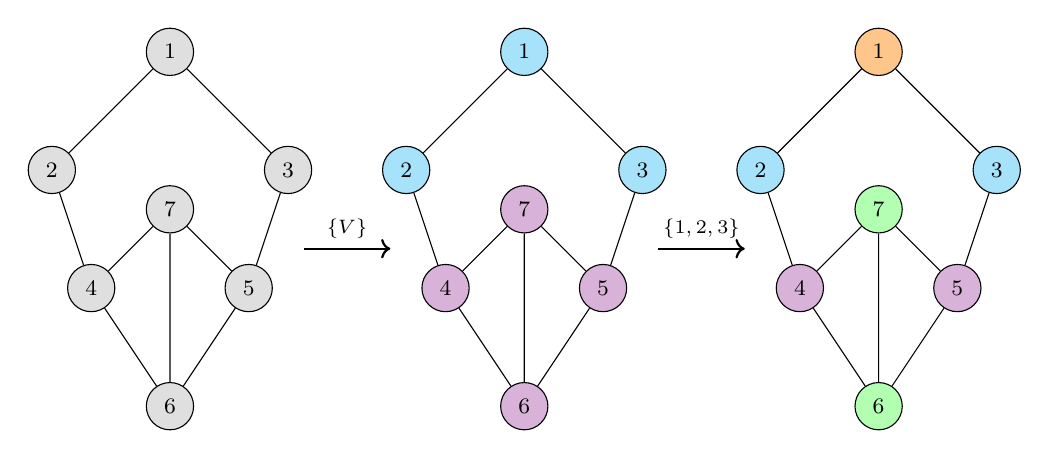
\begin{tikzpicture}
    \tikzset{v/.style={circle, draw, minimum size=6mm, inner sep=0pt, font=\footnotesize}}
    
    % ---- Panel 1: pi_0 (partition initiale) ----
    \begin{scope}
    \node[v, fill=gray!25] (a1) at (0,2.5) {1};
    \node[v, fill=gray!25] (a2) at (-1.5,1) {2};
    \node[v, fill=gray!25] (a3) at (1.5,1) {3};
    \node[v, fill=gray!25] (a4) at (-1,-0.5) {4};
    \node[v, fill=gray!25] (a5) at (1,-0.5) {5};
    \node[v, fill=gray!25] (a6) at (0,-2) {6};
    \node[v, fill=gray!25] (a7) at (0,0.5) {7};
    \draw (a1)--(a2) (a1)--(a3) (a2)--(a4) (a3)--(a5)
          (a4)--(a6) (a5)--(a6) (a4)--(a7) (a5)--(a7) (a6)--(a7);
    \end{scope}
    
    % ---- Panel 2: pi_1 (apres W=V) ----
    \begin{scope}[xshift=4.5cm]
    \node[v, fill=cyan!35] (b1) at (0,2.5) {1};
    \node[v, fill=cyan!35] (b2) at (-1.5,1) {2};
    \node[v, fill=cyan!35] (b3) at (1.5,1) {3};
    \node[v, fill=violet!30] (b4) at (-1,-0.5) {4};
    \node[v, fill=violet!30] (b5) at (1,-0.5) {5};
    \node[v, fill=violet!30] (b6) at (0,-2) {6};
    \node[v, fill=violet!30] (b7) at (0,0.5) {7};
    \draw (b1)--(b2) (b1)--(b3) (b2)--(b4) (b3)--(b5)
          (b4)--(b6) (b5)--(b6) (b4)--(b7) (b5)--(b7) (b6)--(b7);
    \end{scope}
    
    % ---- Panel 3: pi_2 = pi_final (apres W={1,2,3}) ----
    \begin{scope}[xshift=9cm]
    \node[v, fill=orange!45] (c1) at (0,2.5) {1};
    \node[v, fill=cyan!35] (c2) at (-1.5,1) {2};
    \node[v, fill=cyan!35] (c3) at (1.5,1) {3};
    \node[v, fill=violet!30] (c4) at (-1,-0.5) {4};
    \node[v, fill=violet!30] (c5) at (1,-0.5) {5};
    \node[v, fill=green!30] (c6) at (0,-2) {6};
    \node[v, fill=green!30] (c7) at (0,0.5) {7};
    \draw (c1)--(c2) (c1)--(c3) (c2)--(c4) (c3)--(c5)
          (c4)--(c6) (c5)--(c6) (c4)--(c7) (c5)--(c7) (c6)--(c7);
    \end{scope}
    
    % ---- Arrows between panels ----
    \draw[->, thick] (1.7,0) -- node[above, font=\scriptsize] {$\{V\}$} (2.8,0);
    \draw[->, thick] (6.2,0) -- node[above, font=\scriptsize] {$\{1,2,3\}$} (7.3,0);
    \end{tikzpicture}%
    }
    \end{figure}
\end{frame}


\begin{frame}{Fonction: sélection classe}

\begin{figure}[h!]
    \centering
    \resizebox{0.5\textwidth}{!}{%
    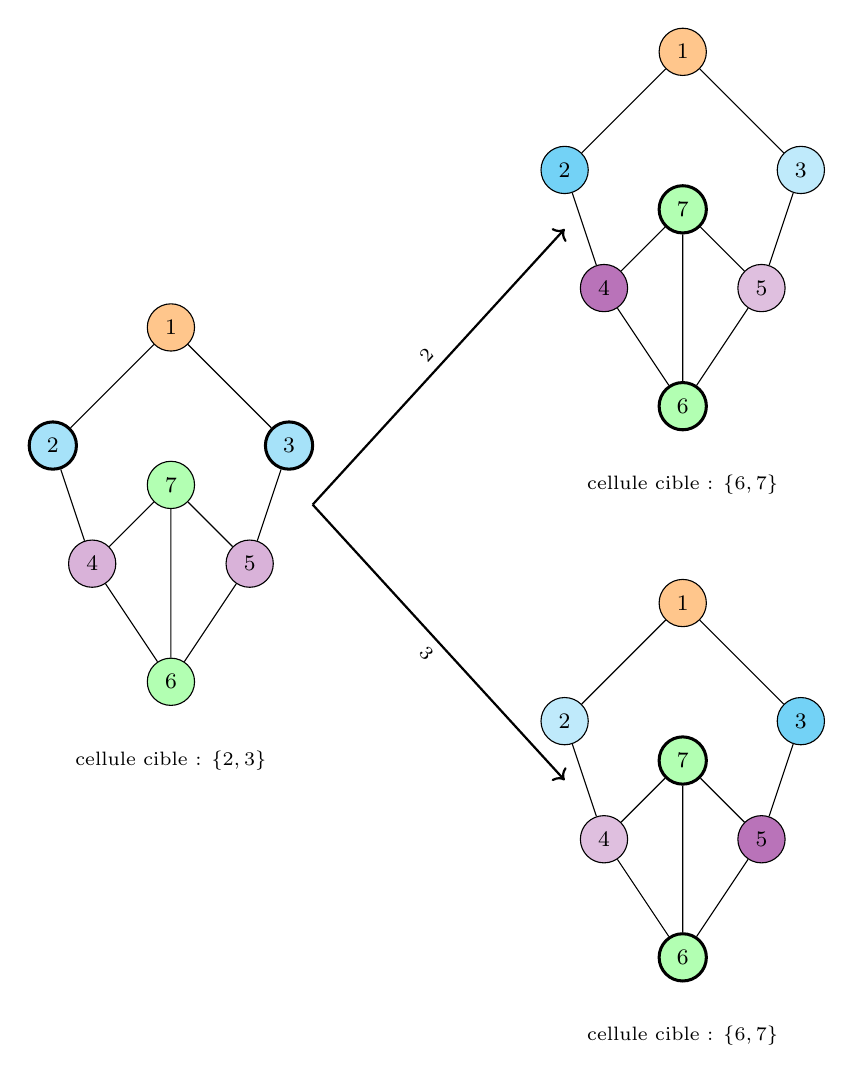
\begin{tikzpicture}
      \tikzset{v/.style={circle, draw, minimum size=6mm, inner sep=0pt, font=\footnotesize}}
      \tikzset{vt/.style={v, line width=1.1pt}}
      
      % ---- Root (gauche) : cellule cible {2,3} mise en evidence ----
      \begin{scope}[xshift=0cm, yshift=0cm]
      \node[v, fill=orange!45] (r1) at (0,2.5) {1};
      \node[vt, fill=cyan!35] (r2) at (-1.5,1) {2};
      \node[vt, fill=cyan!35] (r3) at (1.5,1) {3};
      \node[v, fill=violet!30] (r4) at (-1,-0.5) {4};
      \node[v, fill=violet!30] (r5) at (1,-0.5) {5};
      \node[v, fill=green!30] (r6) at (0,-2) {6};
      \node[v, fill=green!30] (r7) at (0,0.5) {7};
      \draw (r1)--(r2) (r1)--(r3) (r2)--(r4) (r3)--(r5)
            (r4)--(r6) (r5)--(r6) (r4)--(r7) (r5)--(r7) (r6)--(r7);
      \node[align=center, font=\scriptsize] at (0,-3) {cellule cible : $\{2,3\}$};
      \end{scope}
      
      % ---- Enfant haut (droite) : individualiser 2 ----
      \begin{scope}[xshift=6.5cm, yshift=3.5cm]
      \node[v, fill=orange!45] (l1) at (0,2.5) {1};
      \node[v, fill=cyan!55] (l2) at (-1.5,1) {2};
      \node[v, fill=cyan!25] (l3) at (1.5,1) {3};
      \node[v, fill=violet!55] (l4) at (-1,-0.5) {4};
      \node[v, fill=violet!25] (l5) at (1,-0.5) {5};
      \node[vt, fill=green!30] (l6) at (0,-2) {6};
      \node[vt, fill=green!30] (l7) at (0,0.5) {7};
      \draw (l1)--(l2) (l1)--(l3) (l2)--(l4) (l3)--(l5)
            (l4)--(l6) (l5)--(l6) (l4)--(l7) (l5)--(l7) (l6)--(l7);
      \node[align=center, font=\scriptsize] at (0,-3) {cellule cible : $\{6,7\}$};
      \end{scope}
      
      % ---- Enfant bas (droite) : individualiser 3 ----
      \begin{scope}[xshift=6.5cm, yshift=-3.5cm]
      \node[v, fill=orange!45] (s1) at (0,2.5) {1};
      \node[v, fill=cyan!25] (s2) at (-1.5,1) {2};
      \node[v, fill=cyan!55] (s3) at (1.5,1) {3};
      \node[v, fill=violet!25] (s4) at (-1,-0.5) {4};
      \node[v, fill=violet!55] (s5) at (1,-0.5) {5};
      \node[vt, fill=green!30] (s6) at (0,-2) {6};
      \node[vt, fill=green!30] (s7) at (0,0.5) {7};
      \draw (s1)--(s2) (s1)--(s3) (s2)--(s4) (s3)--(s5)
            (s4)--(s6) (s5)--(s6) (s4)--(s7) (s5)--(s7) (s6)--(s7);
      \node[align=center, font=\scriptsize] at (0,-3) {cellule cible : $\{6,7\}$};
      \end{scope}
      
      % ---- Fleches ----
      \draw[->, thick] (1.8,0.25) -- node[above, sloped, font=\scriptsize] {$2$} (5.0,3.75);
      \draw[->, thick] (1.8,0.25) -- node[below, sloped, font=\scriptsize] {$3$} (5.0,-3.25);
      
      \end{tikzpicture}%
    }
    \end{figure}
\end{frame}


\begin{frame}{Fonction: invariant + forme canonique}

    \begin{figure}[h!]
        \centering
        \resizebox{0.9\textwidth}{!}{%
        \input{figTex/slide/slideInvariant.tex}%
        }
        \end{figure}
\end{frame}
            

\begin{frame}{Stratégies d'élagages}

\begin{itemize}
    \item 2 stratégies basées sur l'invariant
    \item 1 stratégie basée sur les automorphismes
    \item Élagage par automorphisme plus performant
    \item Groupe d'automorphisme en cadeau \twemoji{1f381}
\end{itemize}

\end{frame}


\begin{frame}{Élagage par automorphisme}
    \begin{figure}[h!]
        \makebox[\textwidth][l]{%
            \hspace*{-0.8cm}%
            \resizebox{\textwidth}{!}{%
                % Encircle a target cell inline.

\newcommand{\tc}[2][black]{%
\tikz[baseline=(c.base)]{
\node[
    draw=#1,
    text=#1,
    ellipse,
    inner sep=1.5pt,
    outer sep=0pt,
    line width=0.4pt
] (c) {#2};
}%
}

\tikzset{
  stepmark/.style={
    circle, draw=black, fill=white,
    inner sep=0pt, minimum size=4.2mm,
    font=\tiny\bfseries, line width=0.4pt
  },
  steparrow/.style={
    ->,
    dashed,
    line width=0.35pt,
    >=stealth
  }
}

% ---------- Classes de couleur pour le raffinement ----------
% classRoot   : sommet 0 (distingué dès le 1er raffinement)
% classGroup  : sommets encore dans la même classe (non distingués)
% classFirst  : sommet choisi à la 1re individualisation de la branche
% classSecond : sommet choisi à la 2e individualisation de la branche
% classAuto   : sommet distingué automatiquement (dernier de sa classe)

\definecolor{classRoot}{HTML}{2166AC}
\definecolor{classGroup}{HTML}{E08214}
\definecolor{classFirst}{HTML}{B2182B}
\definecolor{classSecond}{HTML}{762A83}
\definecolor{classAuto}{HTML}{1B7837}

\tikzset{
  styGroup/.style ={draw=classGroup,  fill=classGroup!20,  text=classGroup},
  styFirst/.style ={draw=classFirst,  fill=classFirst!20,  text=classFirst,  double},
  stySecond/.style={draw=classSecond, fill=classSecond!20, text=classSecond, double},
  styAuto/.style  ={draw=classAuto,   fill=classAuto!20,   text=classAuto},
}

\newcommand{\ktgraph}[4][black]{%
\begin{tikzpicture}[
    scale=0.42,
    every node/.style={
        circle,
        draw=#1,
        fill=#1!20,
        text=#1,
        inner sep=0pt,
        minimum size=6mm,
        font=\tiny,
        line width=0.5pt
    }
]
\node (g0) at (0,0) {0};

\node[#2] (g1) at (-1.15,1.15) {1};
\node[#3] (g2) at (0,1.55) {2};
\node[#4] (g3) at (1.15,1.15) {3};

\draw[#1] (g0)--(g1);
\draw[#1] (g0)--(g2);
\draw[#1] (g0)--(g3);

\end{tikzpicture}%
}


\begin{tikzpicture}[
    every node/.style={font=\small}
]

% ---------- Initial partition ----------

\node[anchor=north,align=center] (init) at (4.75,14)
{
    \ktgraph[classGroup]{}{}{}
};

% ---------- First refinement ----------

\node[anchor=north,align=center] (root) at (4.75,10)
{
    \ktgraph[classRoot]{styGroup}{styGroup}{styGroup}
};

\draw[
    ->,
    line width=0.5pt
]
(init.south) -- (root.north);


% ---------- Level 1 ----------

\node[anchor=north,align=center] (A) at (-2.25,6)
{
    \ktgraph[classRoot]{styFirst}{styGroup}{styGroup}
};

\node[anchor=north,align=center] (B) at (4.75,6)
{
    \ktgraph[classRoot]{styGroup}{styFirst}{styGroup}
};

\node[
    anchor=north,
    align=center,
    draw=gray,
    dashed,
    rounded corners,
    inner sep=4pt
] (C) at (11.75,6)
{
    \ktgraph[classRoot]{styGroup}{styGroup}{styFirst}\\[2pt]
    {\scriptsize\itshape\color{gray} Élagage $(2\ 3)$}
};


% ---------- Leaves ----------

\node[anchor=north,align=center] (L1) at (-4,1.2)
{
    \ktgraph[classRoot]{styFirst}{stySecond}{styAuto}
};

\node[anchor=north,align=center] (L2) at (-0.5,1.2)
{
    \ktgraph[classRoot]{styFirst}{styAuto}{stySecond}
};

\node[anchor=north,align=center] (L3) at (3,1.2)
{
    \ktgraph[classRoot]{stySecond}{styFirst}{styAuto}
};

\node[
    anchor=north,
    align=center,
    draw=gray,
    dashed,
    rounded corners,
    inner sep=4pt
] (L4) at (6.5,1.2)
{
    \ktgraph[classRoot]{styAuto}{styFirst}{stySecond}\\[2pt]
    {\scriptsize\itshape\color{gray} Élagage $(1\ 3)$}
};

\node[
    anchor=north,
    align=center,
    draw=gray,
    dashed,
    rounded corners,
    inner sep=4pt
] (L5) at (10,1.2)
{
    \ktgraph[gray]{}{}{double}\\[2pt]
    {\scriptsize\itshape\color{gray} Non généré}
};

\node[
    anchor=north,
    align=center,
    draw=gray,
    dashed,
    rounded corners,
    inner sep=4pt
] (L6) at (13.5,1.2)
{
    \ktgraph[gray]{}{double}{double}\\[2pt]
    {\scriptsize\itshape\color{gray} Non généré}
};


% ---------- Edges ----------

\draw (root.south) -- (A.north)
    node[midway,above left] {$1$};

\draw (root.south) -- (B.north)
    node[midway,right] {$2$};

\draw[dashed,gray] (root.south) -- (C.north)
    node[midway,above right,gray] {$3$};


\draw (A.south) -- (L1.north)
    node[midway,left] {$2$};

\draw (A.south) -- (L2.north)
    node[midway,right] {$3$};

\draw (B.south) -- (L3.north)
    node[midway,left] {$1$};

\draw[dashed,gray] (B.south) -- (L4.north)
    node[midway,right,gray] {$3$};

\draw[dashed,gray] (C.south) -- (L5.north)
    node[midway,left,gray] {$1$};

\draw[dashed,gray] (C.south) -- (L6.north)
    node[midway,right,gray] {$2$};


% ---------- Step markers ----------

\node[stepmark] (step1)
    at ($(init.north west)+(-0.3,0.3)$) {1};

\node[stepmark] (step2)
    at ($(L1.north west)+(-0.3,0.3)$) {2};

\node[stepmark] (step3)
    at ($(L2.north east)+(-0.3,0.3)$) {3};

\node[stepmark] (step4)
    at ($(B.north east)+(-0.3,0.3)$) {4};

\node[stepmark] (step5)
    at ($(L3.north west)+(0.3,0.3)$) {5};

\node[stepmark] (step6)
    at ($(L4.north east)+(-1,0.4)$) {6};

\node[stepmark] (step7)
    at ($(C.north east)+(-1,0.4)$) {7};


% ---------- Arrows between step markers ----------

% 1 -> 2
\draw[steparrow]
(step1.south west)
to[out=225,in=135]
(step2.north west);

% 2 -> 3
\draw[steparrow]
(step2.east)
to[out=15,in=165]
(step3.west);

% 3 -> 4
\draw[steparrow]
(step3.north east)
to[out=90,in=200]
(step4.north);

% 4 -> 5
\draw[steparrow]
(step4.south east)
to[out=300,in=135]
(step5.north);

% 5 -> 6
\draw[steparrow]
(step5.east)
to[out=15,in=210]
(step6.south west);

% 6 -> 7
\draw[steparrow]
(step6.north east)
to[out=90,in=250]
(step7.south);

\end{tikzpicture}%
            }%
        }
    \end{figure}
\end{frame}


\section{Conclusion}

\begin{frame}{Conclusion}
\begin{itemize}
    \item \textit{Nauty}: incontournable pour résoudre $\mathrm{IG}$
    \item Fonctionnalités rajoutées entre temps
    \item Implémentation moins bonne  mais respecte bien la logique
\end{itemize}
\end{frame}



\begin{frame}
    
\centering
\Large Merci pour votre attention!

\vspace{1cm}

\Large Questions?

\vspace{1cm}

\email{}

\end{frame}

\section{Annexe}

\begin{frame}{Polynomial-Time Hierarchy}

\begin{figure}[H]
    \centering
    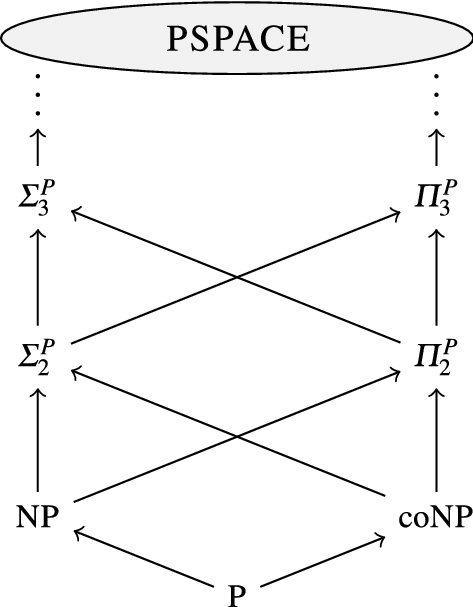
\includegraphics[width=0.5\linewidth]{imgs/Complexity-classes-the-polynomial-hierarchy-Stockmeyer-1976.png}
\end{figure}
    
\end{frame}

\begin{frame}{Complexité supplémentaire}

\begin{itemize}
    \item Probablement pas \NPC{} car ETH
    \item avant 2016: meilleur algorithme en $e^{\mathcal{O}(\sqrt{n \log n})}$
    \item Algorithme quasi-polynomial, purement théorique pour l'instant
    \item appartient à \SPP{}
    \item Différentes complexités en fonction de la famille de graphe
\end{itemize}    
\end{frame}

\begin{frame}{Colour refinement (1/2)}


        \begin{algorithmic}[1]
        
            \State \textbf{Input:} A graph $G=(V,E)$
            
            \State \textbf{Initialisation:} Assign the same colour to every vertex.
        
            \Repeat
                \State \textbf{Refinement Step:}
                
                \ForAll{vertices $v,w$ with the same colour}
                    \If{$v$ and $w$ have different numbers of neighbours in some colour class}
                        \State Assign different colours to $v$ and $w$.
                    \EndIf
                \EndFor
                
            \Until{the colouring is stable}
        
            \State \textbf{Return:} the stable colouring.
        
        \end{algorithmic}

\end{frame}

\begin{frame}{Colour refinement (2/2)}

\begin{itemize}
    \item \textit{Nauty} se base dessus mais avec des différences
    \item Identifie un graphe $G$ s’il permet de le distinguer de tous les graphes non isomorphes à $G$
    \item Nécessaire mais pas suffisante
\end{itemize}
    
\end{frame}

\begin{frame}{Différents types d'invariants}

\begin{itemize}
    \item Nombre de triangle par couleur: $O(n \cdot d^2)$
    \item 2-chemin depuis une couleur: $O(n+m)$
    \item Triple par couleur: $O(n^4)$
    \item Invariant sommet par \textit{Nauty}
    \item Changement d'invariant à faire
\end{itemize}
    
\end{frame}

\begin{frame}{Stratégie basée sur l'invariant}
    \begin{block}{$\mathcal{P}_A$}
        Éliminer les branches dont l’invariant ne peut pas atteindre la valeur maximale: à chaque niveau de l’arbre, on conserve le meilleur invariant trouvé jusqu’à présent, et tout autre nœud situé au même niveau dont l’invariant est strictement inférieur voit sa branche élaguée.
    \end{block}

    \begin{block}{$\mathcal{P}_B$}
        Les noeuds sont comparés à un nœud de référence (noeud sur le chemin de la première feuille rencontrée). Si les deux invariants diffèrent, le sous-arbre courant est élagué. L’objectif n’est pas réellement de trouver le meilleur invariant, mais plutôt de trouver des nouveaux automorphismes.
    \end{block}

    \begin{alertblock}{En pratique}
        Il faut que les 2 conditions soient combinées pour élaguer le noeud.
    \end{alertblock}
    \end{frame}


\begin{frame}{Exemple automorphisme}

    \centering
    \begin{tabular}{@{}ccc@{}}
      \Kautoexample{leafA}{leafB}{leafC}{\mathrm{id}}     &
      \Kautoexample{leafB}{leafA}{leafC}{(1\,2)}          &
      \Kautoexample{leafC}{leafB}{leafA}{(1\,3)}          \\[0.5cm]
      \Kautoexample{leafA}{leafC}{leafB}{(2\,3)}          &
      \Kautoexample{leafB}{leafC}{leafA}{(1\,2\,3)}       &
      \Kautoexample{leafC}{leafA}{leafB}{(1\,3\,2)}
    \end{tabular}
  
    \vspace{0.4cm}

\end{frame}

\begin{frame}{Schreier-Sims}

    \begin{itemize}
        \item Utilisé pour $\mathcal{P}_C$
        \item Garde le groupe d'automorphisme
        \item Complexité en $O(n^2 \log^3 |G| + tn \log |G|)$
        \item Existe une version randomisée:  $O(n^3 \log^c n)$
    \end{itemize}
        
    \end{frame}



\begin{frame}{Experimentation}

\begin{itemize}
    \item Plusieurs experimentation faites
    \item Temps d'éxécution: avec élagage vs sans
    \item 6 types de graphes
    \item Performance sur l'élagage
    \item Légende graphiques ci-dessous
    \item absice = nombre de sommets; ordonné = temps en ms
\end{itemize}

\legendeInvariants{}
    
\end{frame}

\begin{frame}{Temps d'éxécution (1/6)}
    \begin{columns}[c] % [c] = alignement vertical centré des colonnes
        \begin{column}{0.42\textwidth}
            \centering
            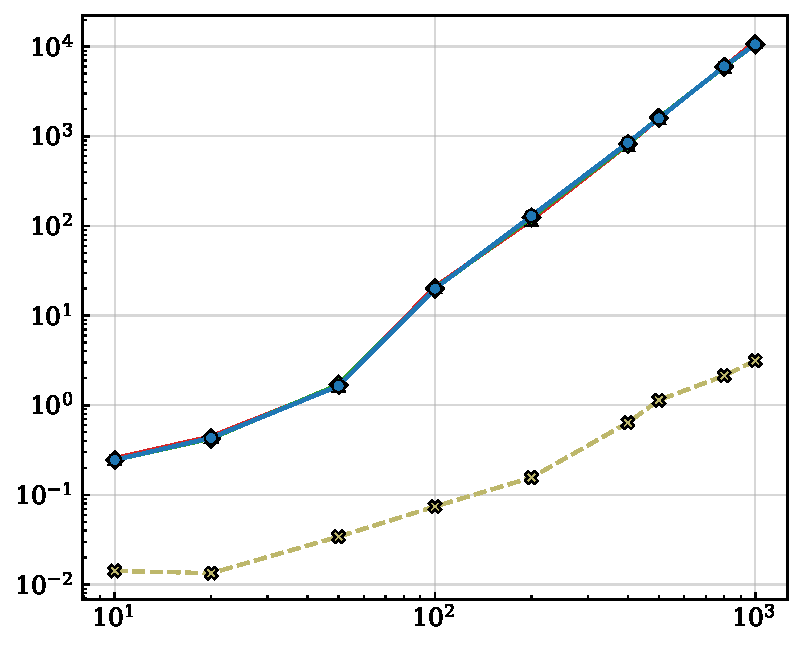
\includegraphics[width=\linewidth]{imgs/test/bipartite.pdf}
        \end{column}
        \begin{column}{0.42\textwidth}
            \centering
            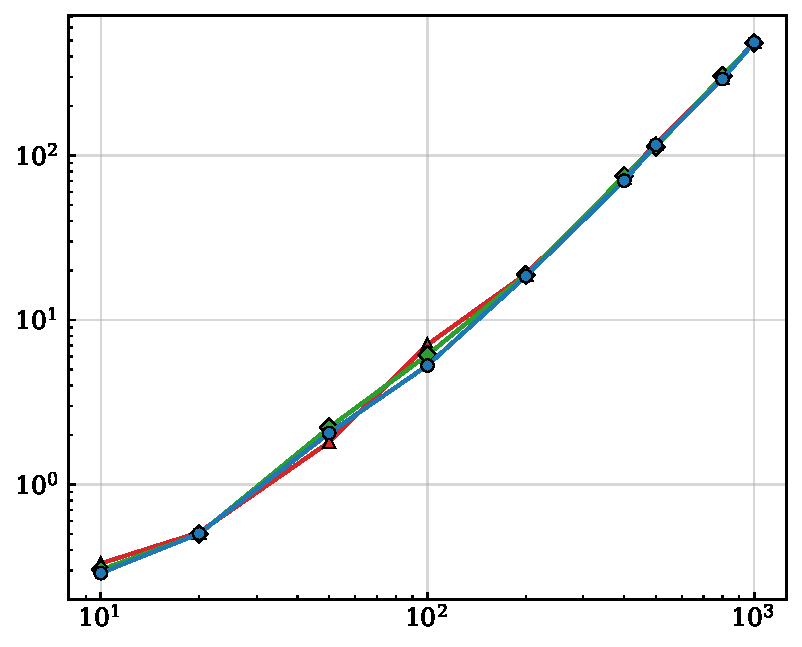
\includegraphics[width=\linewidth]{imgs/WithoutPrunning/bipartiteWP.pdf}
        \end{column}
    \end{columns}
 
    \vspace{1em}
    \centering
    \small Biparti
\end{frame}


\begin{frame}{Temps d'éxécution (2/6)}
    \begin{columns}[c] % [c] = alignement vertical centré des colonnes
        \begin{column}{0.42\textwidth}
            \centering
            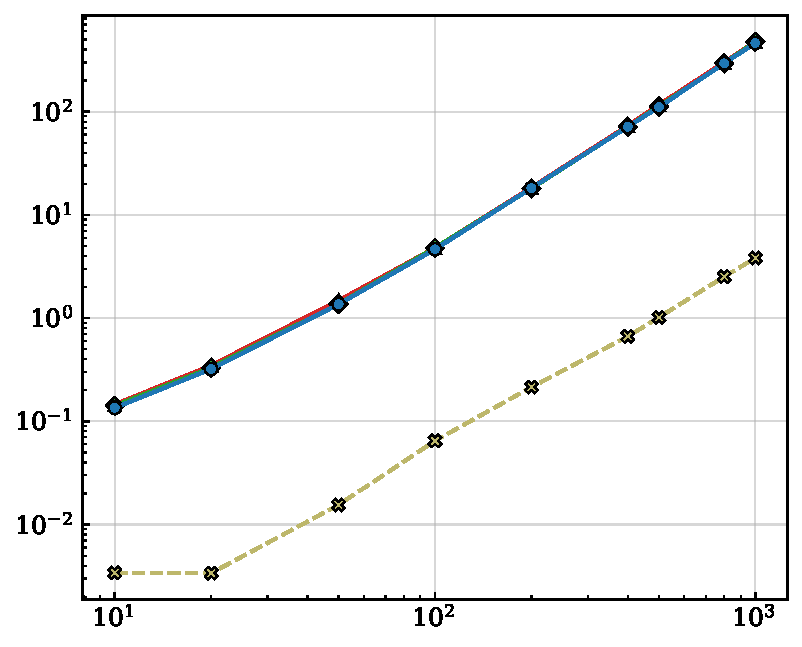
\includegraphics[width=\linewidth]{imgs/test/random.pdf}
        \end{column}
        \begin{column}{0.42\textwidth}
            \centering
            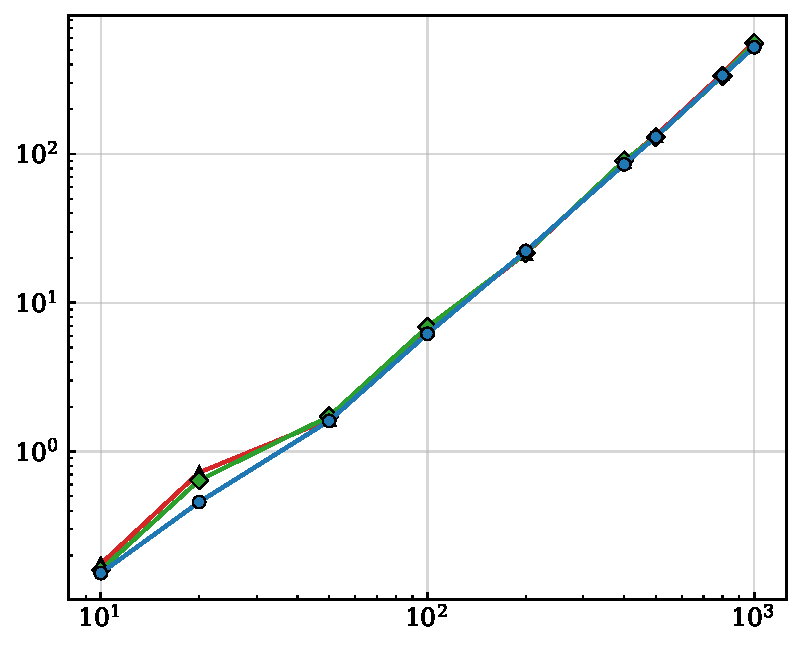
\includegraphics[width=\linewidth]{imgs/WithoutPrunning/randomWP.pdf}
        \end{column}
    \end{columns}
 
    \vspace{1em}
    \centering
    \small graphe aléatoire $\mathcal{G}(n, 1/2)$
\end{frame}


\begin{frame}{Temps d'éxécution (3/6)}
    \begin{columns}[c] % [c] = alignement vertical centré des colonnes
        \begin{column}{0.42\textwidth}
            \centering
            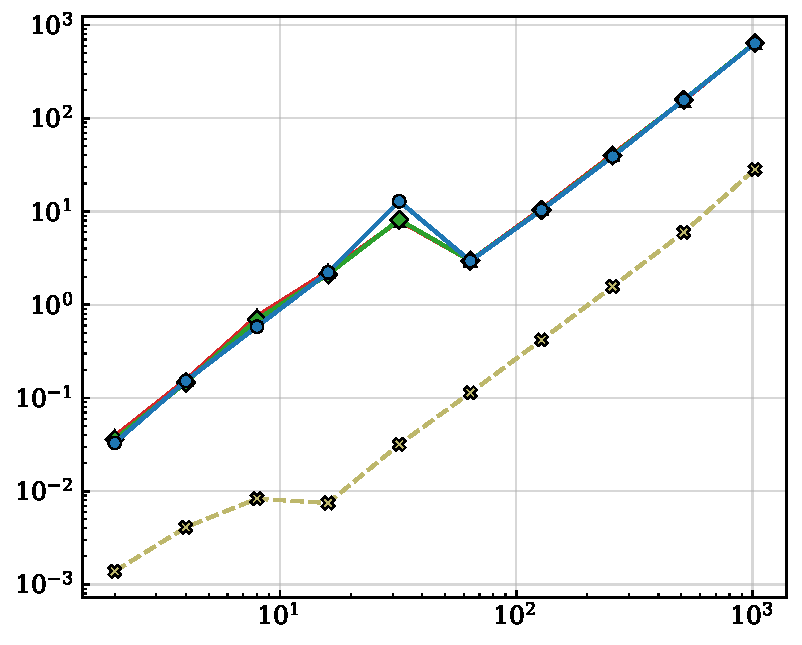
\includegraphics[width=\linewidth]{imgs/test/hypercube.pdf}
        \end{column}
        \begin{column}{0.42\textwidth}
            \centering
            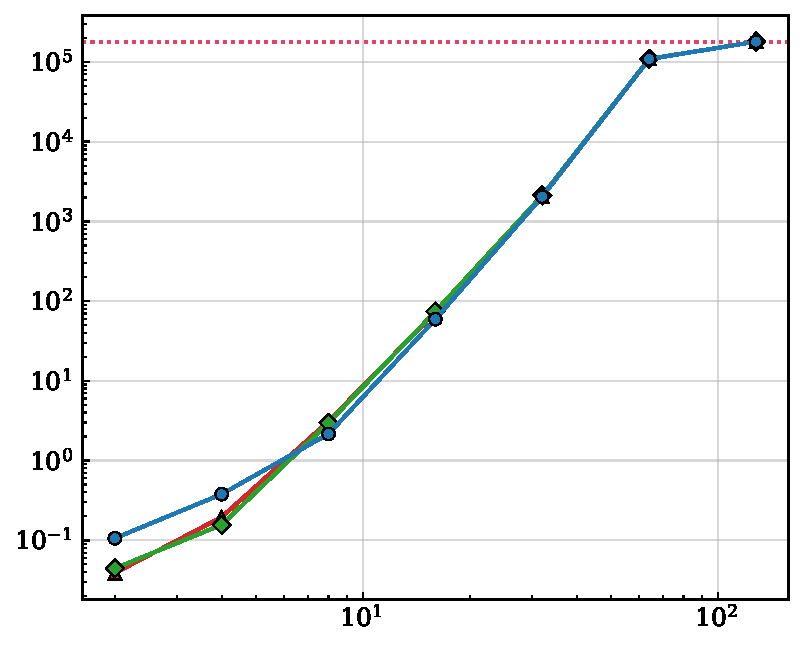
\includegraphics[width=\linewidth]{imgs/WithoutPrunning/hypercubeWP.pdf}
        \end{column}
    \end{columns}
 
    \vspace{1em}
    \centering
    \small Hypercube
\end{frame}

\begin{frame}{Temps d'éxécution (4/6)}
    \begin{columns}[c] % [c] = alignement vertical centré des colonnes
        \begin{column}{0.42\textwidth}
            \centering
            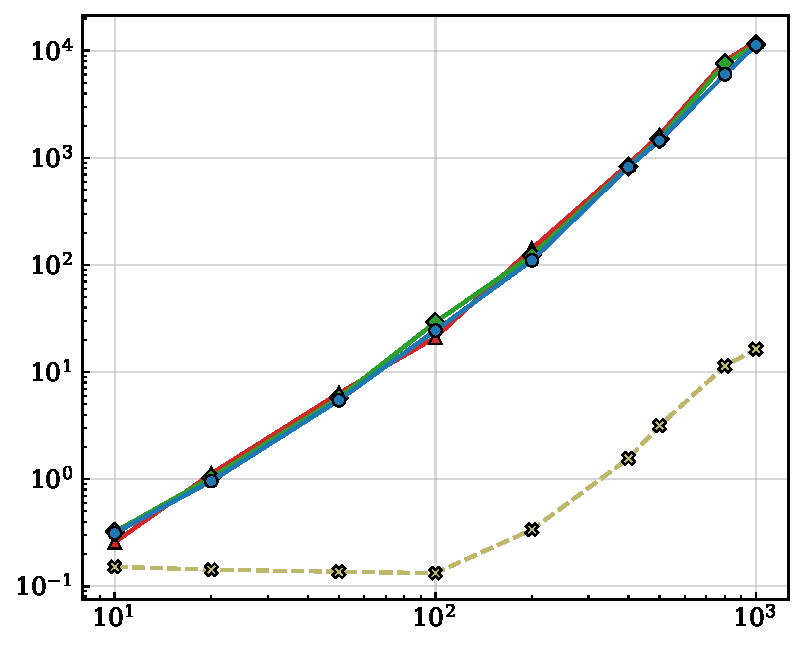
\includegraphics[width=\linewidth]{imgs/test/trees.pdf}
        \end{column}
        \begin{column}{0.42\textwidth}
            \centering
            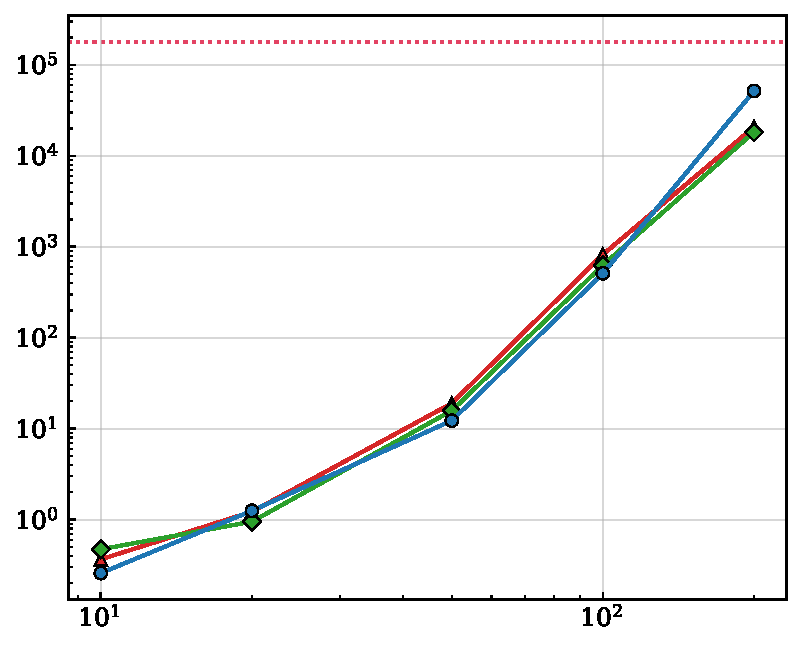
\includegraphics[width=\linewidth]{imgs/WithoutPrunning/treesWP.pdf}
        \end{column}
    \end{columns}
 
    \vspace{1em}
    \centering
    \small Arbres
\end{frame}

\begin{frame}{Temps d'éxécution (5/6)}
    \begin{columns}[c] % [c] = alignement vertical centré des colonnes
        \begin{column}{0.42\textwidth}
            \centering
            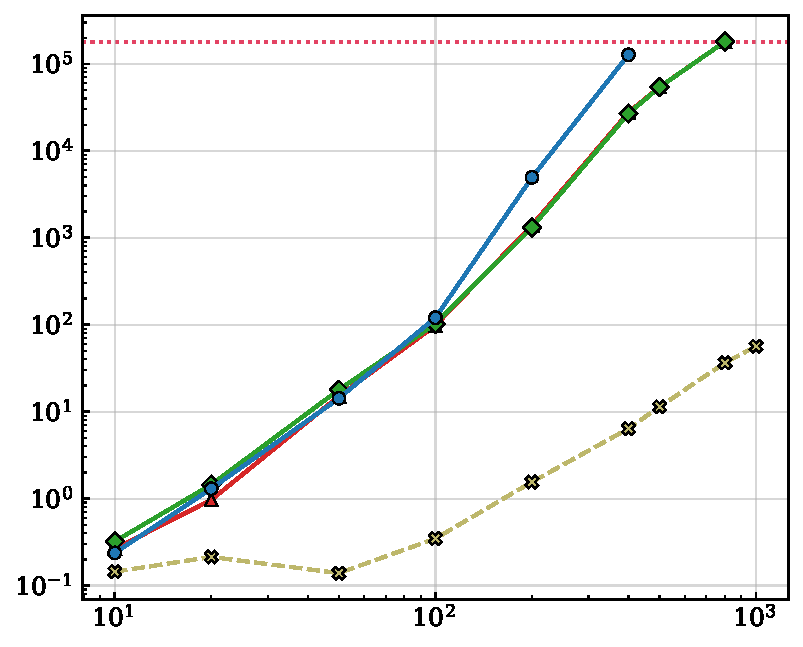
\includegraphics[width=\linewidth]{imgs/test/sparse.pdf}
        \end{column}
        \begin{column}{0.42\textwidth}
            \centering
            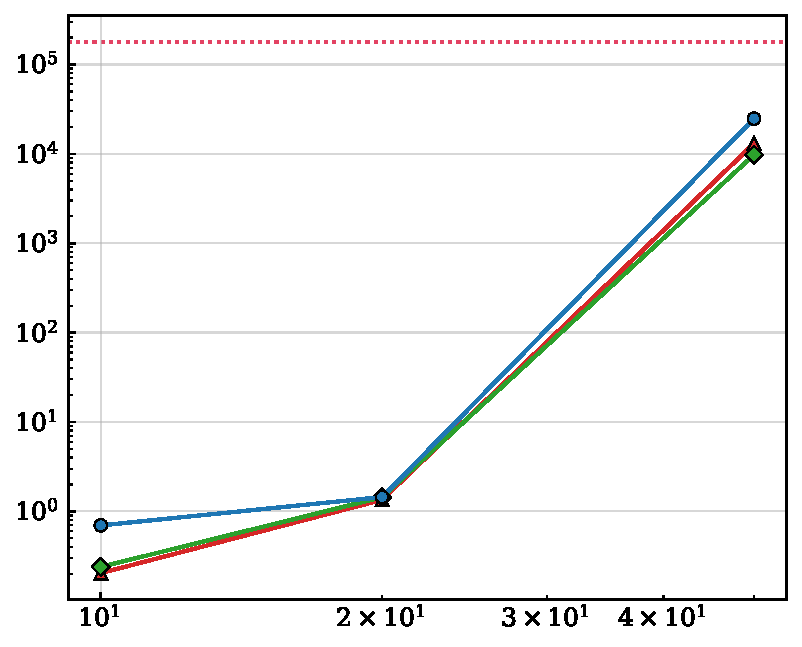
\includegraphics[width=\linewidth]{imgs/WithoutPrunning/sparseWP.pdf}
        \end{column}
    \end{columns}
 
    \vspace{1em}
    \centering
    \small Biparti
\end{frame}

\begin{frame}{Temps d'éxécution (6/6)}
    \begin{columns}[c] % [c] = alignement vertical centré des colonnes
        \begin{column}{0.42\textwidth}
            \centering
            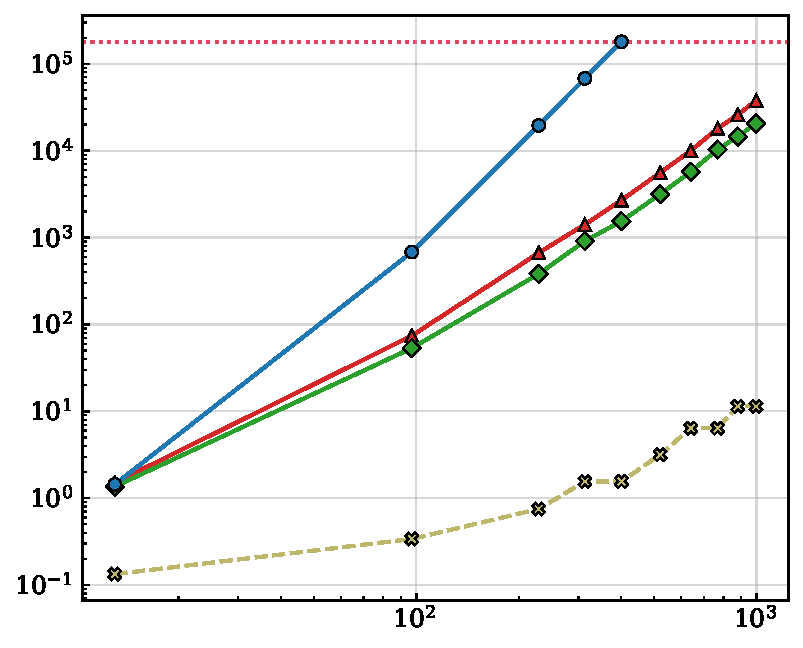
\includegraphics[width=\linewidth]{imgs/test/paley.pdf}
        \end{column}
        \begin{column}{0.42\textwidth}
            \centering
            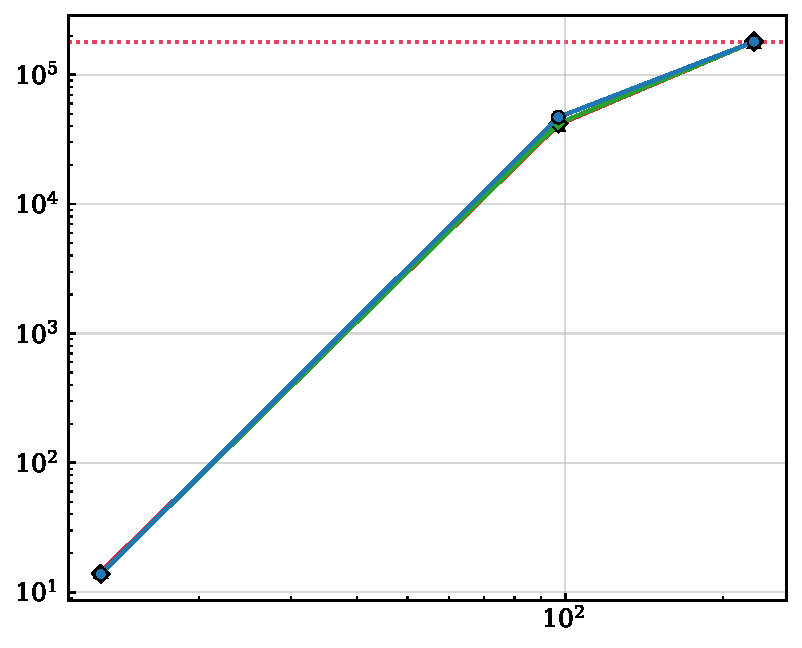
\includegraphics[width=\linewidth]{imgs/WithoutPrunning/paleyWP.pdf}
        \end{column}
    \end{columns}
 
    \vspace{1em}
    \centering
    \small Paley
\end{frame}

\begin{frame}{Performance élagage (exemple arbre)}
    \begin{figure}[H]
        \centering
        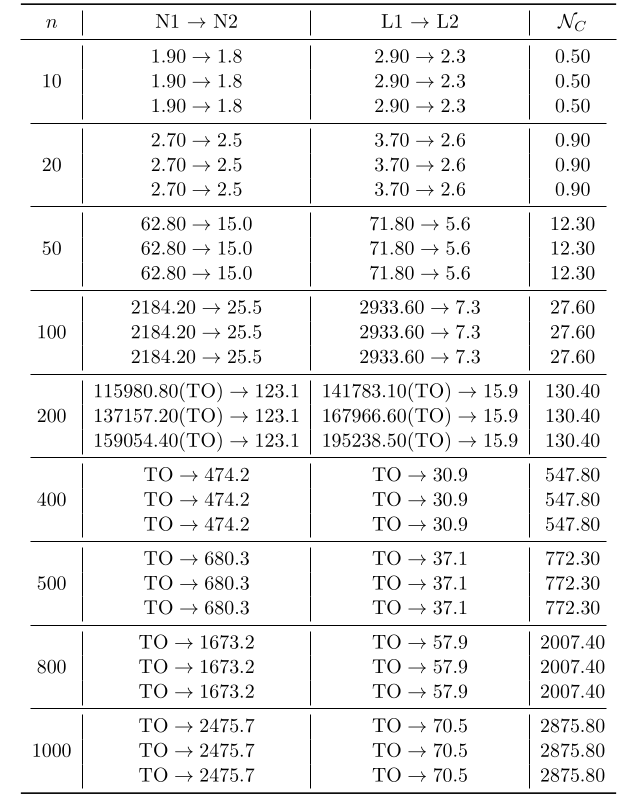
\includegraphics[width=0.5\linewidth]{imgs/slide/Image collée.png}
    \end{figure}

\end{frame}
\end{document}

